\chapter{DESAIN DAN IMPLEMENTASI SISTEM}
\vspace{1ex}

\section*{}
	Penelitian ini dilaksanakan sesuai dengan desain sistem berikut dengan implementasinya. Desain sistem merupakan konsep dari pembuatan dan perancangan infrastruktur kemudian diwujudkan dalam bentuk blok-blok alur yang harus dikerjakan. Pada bagian implementasi merupakan pelaksanaan teknis untuk setiap blok pada desain sistem.
\vspace{1ex}

\section{Desain Sistem}
\vspace{1ex}

	\par Tugas akhir ini merupakan penelitian dalam bidang visi komputer yang bertujuan untuk mendeteksi pelanggaran pengendara bermotor yang tidak menggunakan helm berbasis Deep Learning. Sistem deteksi ini memanfaatkan data training yang diambil dari video rekaman IP Camera yang terpasang diseluruh jalan Kota Surabaya oleh Dinas Perhubungan Kota Surabaya.
\begin{figure}[H]
	\captionsetup{justification=centering}
	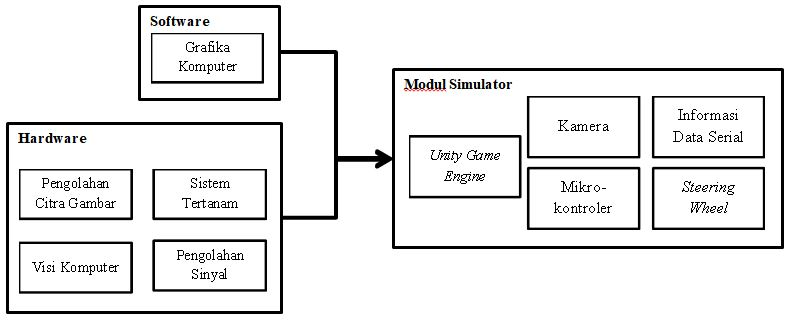
\includegraphics[scale=0.55]{img/cakupanTA.JPG}
	\caption{Blok Diagram Cakupan Disiplin Ilmu Tugas Akhir}
	\label{fig: 3_1}
\end{figure}
\vspace{1ex}

\section{Alur Kerja}
\vspace{1ex}

	\par Tugas akhir ini merupakan penelitian dalam bidang visi komputer yang bertujuan untuk mendeteksi pelanggaran pengendara bermotor yang tidak menggunakan helm berbasis Deep Learning. Sistem deteksi ini memanfaatkan data training yang diambil dari video rekaman IP Camera yang terpasang diseluruh jalan Kota Surabaya oleh Dinas Perhubungan Kota Surabaya.
\begin{figure}[H]
	\captionsetup{justification=centering}
	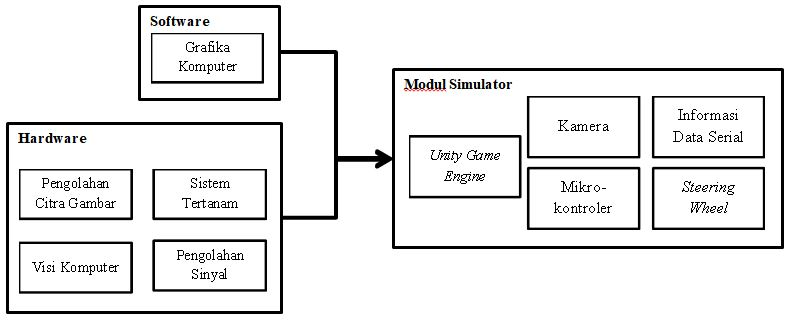
\includegraphics[scale=0.55]{img/cakupanTA.JPG}
	\caption{Blok Diagram Cakupan Disiplin Ilmu Tugas Akhir}
	\label{fig: 3_1}
\end{figure}
\vspace{1ex}

\section{Pelabelan Objek}
\vspace{1ex}

	\par Tugas akhir ini merupakan penelitian dalam bidang visi komputer yang bertujuan untuk mendeteksi pelanggaran pengendara bermotor yang tidak menggunakan helm berbasis Deep Learning. Sistem deteksi ini memanfaatkan data training yang diambil dari video rekaman IP Camera yang terpasang diseluruh jalan Kota Surabaya oleh Dinas Perhubungan Kota Surabaya.
\begin{figure}[H]
	\captionsetup{justification=centering}
	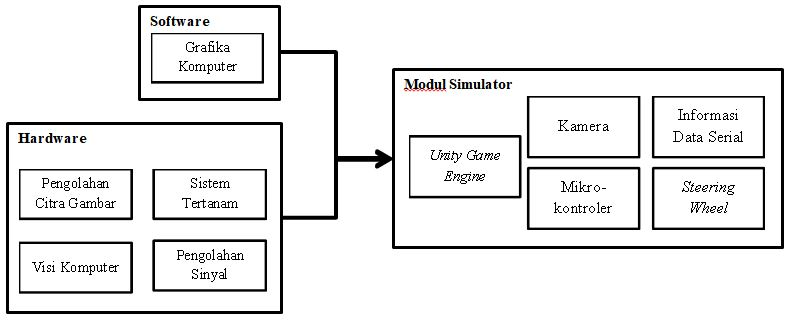
\includegraphics[scale=0.55]{img/cakupanTA.JPG}
	\caption{Blok Diagram Cakupan Disiplin Ilmu Tugas Akhir}
	\label{fig: 3_1}
\end{figure}
\vspace{1ex}
    
\section{Proses \textit{Training} Dataset}
\vspace{1ex}

	\par Tugas akhir ini merupakan penelitian dalam bidang visi komputer yang bertujuan untuk mendeteksi pelanggaran pengendara bermotor yang tidak menggunakan helm berbasis Deep Learning. Sistem deteksi ini memanfaatkan data training yang diambil dari video rekaman IP Camera yang terpasang diseluruh jalan Kota Surabaya oleh Dinas Perhubungan Kota Surabaya.
\begin{figure}[H]
	\captionsetup{justification=centering}
	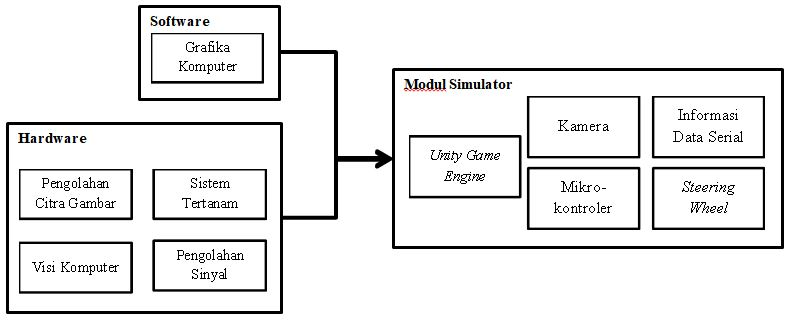
\includegraphics[scale=0.55]{img/cakupanTA.JPG}
	\caption{Blok Diagram Cakupan Disiplin Ilmu Tugas Akhir}
	\label{fig: 3_1}
\end{figure}
\vspace{1ex}

\section{Pengembangan Sistem Deteksi}
\vspace{1ex}

	\par Tugas akhir ini merupakan penelitian dalam bidang visi komputer yang bertujuan untuk mendeteksi pelanggaran pengendara bermotor yang tidak menggunakan helm berbasis Deep Learning. Sistem deteksi ini memanfaatkan data training yang diambil dari video rekaman IP Camera yang terpasang diseluruh jalan Kota Surabaya oleh Dinas Perhubungan Kota Surabaya.
\begin{figure}[H]
	\captionsetup{justification=centering}
	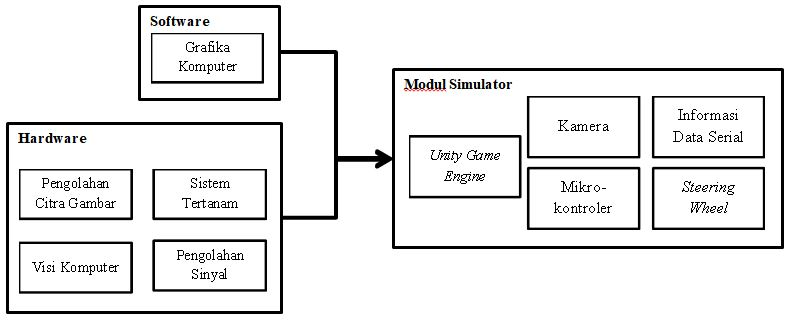
\includegraphics[scale=0.55]{img/cakupanTA.JPG}
	\caption{Blok Diagram Cakupan Disiplin Ilmu Tugas Akhir}
	\label{fig: 3_1}
\end{figure}
\vspace{1ex}

\section{Analisa Performa}
\vspace{1ex}

	\par Tugas akhir ini merupakan penelitian dalam bidang visi komputer yang bertujuan untuk mendeteksi pelanggaran pengendara bermotor yang tidak menggunakan helm berbasis Deep Learning. Sistem deteksi ini memanfaatkan data training yang diambil dari video rekaman IP Camera yang terpasang diseluruh jalan Kota Surabaya oleh Dinas Perhubungan Kota Surabaya.
\begin{figure}[H]
	\captionsetup{justification=centering}
	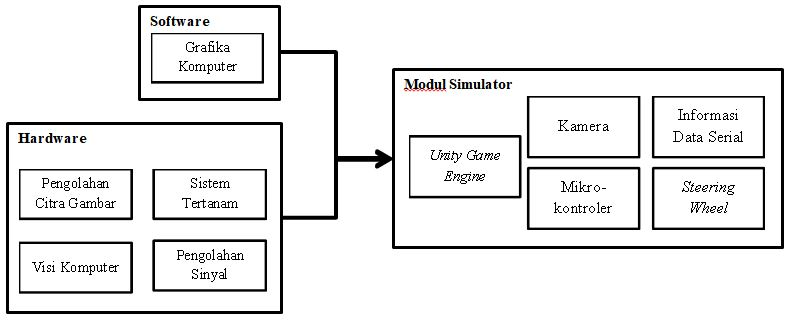
\includegraphics[scale=0.55]{img/cakupanTA.JPG}
	\caption{Blok Diagram Cakupan Disiplin Ilmu Tugas Akhir}
	\label{fig: 3_1}
\end{figure}
\vspace{1ex}